\section{CHƯƠNG 5: CÔNG CỤ HỖ TRỢ VIẾT KỊCH BẢN CHO VIDEO TIKTOK} \label{sec:scriptwriting}

Quy trình tạo kịch bản video TikTok được xây dựng theo hướng \textbf{few-shot \textit{prompt}ing} trên nền tảng mô hình \textbf{Gemini}. Hệ thống phân tích mô tả đầu vào từ người dùng để đề xuất bộ lọc phù hợp, sau đó lựa chọn một nhóm video tương đồng từ tập dữ liệu đã annotate. Các video mẫu này được đưa trực tiếp vào \textit{prompt} dưới dạng ví dụ minh hoạ để mô hình sinh ra kịch bản thô dạng đoạn văn. Kịch bản sau đó được đưa vào một bước xử lý thứ hai để tự động phân đoạn và gắn nhãn nội dung, tạo thành bản kịch bản hoàn chỉnh có cấu trúc.

\subsection{Trích xuất đặc trưng nội dung}

\begin{table}[ht]
\centering
\footnotesize
\renewcommand{\arraystretch}{1.4}
\begin{tabular}{|>{\arraybackslash}m{3.5cm}|p{12.5cm}|}
\hline
\textbf{Tên trường} & \textbf{Mô tả} \\
\hline
\texttt{categories} & Thể loại chính của video. Bắt buộc. Nếu không liên quan đến ẩm thực, chỉ trả về trường này với giá trị ``Không liên quan ẩm thực''. \\
\hline
\texttt{structure\_style} & Các kỹ thuật trình bày nội dung như kể chuyện, mô tả đặc điểm, hướng dẫn, v.v.. \\
\hline
\texttt{hook\_type} & Cách mở đầu video nhằm thu hút người xem (ví dụ: gây tò mò, giật tít vào thẳng vấn đề, v.v.). \\
\hline
\texttt{tone\_of\_voice} & Giọng điệu và cảm xúc của người nói, như hài hước, chân thành, thân thiện, v.v.. \\
\hline
\texttt{pacing} & Nhịp độ triển khai video: nhanh, chậm hoặc thay đổi. \\
\hline
\texttt{has\_cta}, \texttt{cta\_type} & Cho biết video có kêu gọi hành động không và nếu có thì đó là loại nào (ví dụ: follow, bình luận, chia sẻ, ghé quán, v.v.). \\
\hline
\texttt{content\_style} & Phong cách tổng thể của nội dung: Gen Z, chuyên nghiệp, truyền thống, v.v.. \\
\hline
\texttt{audience\_target} & Nhóm khán giả mục tiêu mà video hướng tới (ví dụ: học sinh, dân văn phòng, người ăn chay, v.v.). \\
\hline
\end{tabular}
\caption{Các trường được trích xuất từ nội dung video}
\label{tab:extraction_fields}
\end{table}

Để phục vụ cho quá trình lọc video mẫu và sinh kịch bản, nhóm đã tiến hành trích xuất các đặc trưng nội dung từ \textit{mô tả} và \textit{transcript} của từng video TikTok. Việc trích xuất được thực hiện bằng mô hình ngôn ngữ lớn (LLM) với \textbf{\textit{prompt} định hướng chi tiết}, nhằm gán nhãn cho từng trường nội dung theo một \textbf{schema chuẩn hoá}.

Trong giai đoạn đầu, nhóm không giới hạn tập nhãn cố định mà cho phép Gemini được \textbf{tự do gán nhãn} cho các trường nội dung (\textit{free-form annotation}), không áp đặt trước số lượng hay tên nhãn cụ thể cho mỗi trường. Việc này cho phép thu thập linh hoạt các kiểu biểu hiện phong phú trong nội dung video thực tế. Sau đó, hệ thống tiến hành \textbf{thống kê các nhãn có số lượng video cao nhất ở mỗi trường} và thực hiện một vài bước \textbf{tinh chỉnh thủ công}, từ đó xác định một tập nhãn phổ biến và ổn định để sử dụng nhất quán trong toàn bộ \textit{pipeline}.

Để đảm bảo sự đồng nhất trong định dạng và nội dung đầu ra khi \textit{prompt} với Gemini, nhóm đã sử dụng một \textbf{response schema JSON} làm chuẩn. Schema này quy định rõ tên các trường được trích xuất, kiểu dữ liệu, danh sách các nhãn hợp lệ (nếu có), cũng như yêu cầu về tính bắt buộc của từng trường. Nhờ đó, mô hình có thể sinh đầu ra \textbf{đúng cấu trúc và dễ dàng xử lý} tiếp trong các bước lọc và sinh kịch bản. Một số trường nội dung quan trọng được trình bày trong Bảng~\ref{tab:extraction_fields}.

\subsection{Lọc video tương đồng theo mô tả người dùng}

Sau khi người dùng nhập mô tả tự nhiên về nội dung video muốn tạo, hệ thống sẽ tiến hành phân tích mô tả để gán nhãn cho các trường nội dung đã chuẩn hoá trước đó. Quá trình này được thực hiện bằng mô hình Gemini, sử dụng \textit{prompt} riêng kèm theo \textbf{response schema} định nghĩa các trường như \texttt{categories}, \texttt{structure\_style}, \texttt{tone\_of\_voice}, v.v.. Ngoài ra, trong quá trình xử lý mô tả đầu vào, hệ thống cũng thực hiện \textbf{trích xuất thời lượng mong muốn} nếu người dùng có đề cập đến (ví dụ: ``video khoảng 30 giây'', ``tầm 1 phút rưỡi'', v.v.). Thời lượng này sẽ được sử dụng trong bước sinh kịch bản để kiểm soát độ dài hợp lý của nội dung đầu ra.

Các nhãn nội dung được sinh từ mô tả sẽ được sử dụng như điều kiện lọc để chọn ra các video có nội dung tương đồng trong tập dữ liệu đã annotate. Việc lọc được thực hiện bởi hàm \texttt{filter\allowbreak\_by\allowbreak\_multiple\allowbreak\_labels\allowbreak\_unified}, theo cơ chế:

\begin{enumerate}
    \item Ban đầu áp dụng toàn bộ các điều kiện lọc.
    \item Nếu không đủ số lượng video (mặc định là 20), hệ thống sẽ dần dần \textbf{nới lỏng điều kiện} theo thứ tự ưu tiên: nới nhãn trong từng trường, sau đó loại bỏ cả trường (trừ \texttt{categories}).
    \item Quá trình dừng lại khi đạt đủ số lượng video tối thiểu hoặc khi đã nới tối đa có thể.
\end{enumerate}

\noindent Nhờ cơ chế \textit{lọc mềm}, hệ thống có thể tìm được một tập video mẫu có mức độ tương đồng cao với ý tưởng đầu vào của người dùng, ngay cả khi mô tả ban đầu quá cụ thể hoặc hiếm gặp trong dữ liệu.

Nếu kết quả gán nhãn ban đầu xác định rằng video không liên quan đến ẩm thực (giá trị ``Không liên quan ẩm thực'' trong trường \texttt{categories}), quy trình sẽ dừng và yêu cầu người dùng nhập lại mô tả phù hợp.

\subsection{Sinh kịch bản thô từ video mẫu}

Sau khi lọc được tập video có nội dung tương đồng với mô tả đầu vào, hệ thống tiến hành bước sinh kịch bản thô bằng phương pháp \textbf{few-shot prompting}. Cụ thể, hệ thống chọn tối đa \textbf{20 video mẫu} làm ví dụ đầu vào để hướng dẫn mô hình sinh ra một kịch bản mới phù hợp với bối cảnh yêu cầu. Việc sử dụng số lượng ví dụ lớn (20-shot) giúp mô hình có đủ dữ liệu tham chiếu để tái tạo phong cách nội dung phổ biến trong các video TikTok ẩm thực.
Tập video mẫu được chọn dựa trên một công thức chấm điểm đơn giản, kết hợp giữa \textbf{mức độ phổ biến} và \textbf{độ gần thời gian} của video. Cụ thể, điểm số được tính theo công thức:
\[
\text{Score} = \frac{\text{Lượt xem}}{(\text{Số ngày kể từ ngày đăng} + 1)^{\alpha}}, \quad \alpha = 0.7
\]
Công thức này \textbf{ưu tiên các video có lượt xem cao}, đồng thời điều chỉnh theo thời gian để \textbf{tăng trọng số cho những nội dung mới} được đăng gần đây. Từ danh sách được sắp xếp theo điểm số giảm dần, hệ thống chọn ra 20 video đầu tiên để làm ví dụ minh hoạ trong \textit{prompt}.

Để giới hạn độ dài hợp lý cho kịch bản đầu ra, hệ thống ước lượng \textbf{word count mục tiêu} dựa trên hai nguồn:
\begin{itemize}
    \item Nếu người dùng có đề cập đến \textbf{thời lượng mong muốn} trong phần mô tả đầu vào, hệ thống sẽ trích xuất con số này và chuyển đổi thành số từ (\textit{word count}) tương ứng.
    \item Nếu không có thông tin rõ ràng từ mô tả, hệ thống sử dụng \textbf{thời lượng trung bình của các video mẫu} đã lọc và nhân với \textbf{tốc độ nói trung bình} để tính ra số từ tối ưu.
\end{itemize}

Việc kiểm soát độ dài bằng word count giúp kịch bản sinh ra phù hợp với nhịp độ thực tế của video TikTok, tránh việc mô hình tạo nội dung quá dài hoặc quá ngắn so với kỳ vọng. Đây là một điểm then chốt trong pipeline, đảm bảo đầu ra có tính khả dụng cao và nhất quán với trải nghiệm người dùng.

Từ phần mô tả gốc và các ví dụ đã chọn, mô hình sẽ sinh ra một đoạn văn liền mạch, được xem là \textbf{kịch bản thô ban đầu}. Đoạn này chưa có cấu trúc rõ ràng, không phân chia các phần nội dung cụ thể như mở bài, nội dung chính hay CTA, nhưng vẫn đảm bảo đúng tone, nhịp điệu và đặc điểm của các video TikTok ẩm thực phổ biến.


\subsection{Định dạng lại kịch bản có cấu trúc}

Sau khi sinh được kịch bản thô từ mô tả và các video mẫu tương đồng, hệ thống tiếp tục định dạng lại nội dung đầu ra thành một cấu trúc rõ ràng hơn, nhằm phục vụ cho các bước hậu kỳ và sản xuất video sau này.

Bước này được thực hiện bằng mô hình Gemini cùng với một \textbf{prompt chuyên biệt}, trong đó yêu cầu mô hình:
\begin{itemize}
    \item Chuyển kịch bản dạng \textit{plain} thành một JSON hợp lệ theo schema đã định nghĩa.
    \item Giữ nguyên lời thoại gốc, không viết lại nội dung.
    \item Chia nhỏ theo từng phần như mở đầu, mô tả món, cảm nhận, CTA, v.v..
    \item Dựa vào thời lượng ước tính của video, các đoạn mô tả mẫu và danh sách hashtag phổ biến để sinh phần mô tả video.
\end{itemize}

Mô hình được yêu cầu tạo ra một \textbf{kịch bản có chú thích rõ ràng cho từng phần nội dung}, dựa trên một \textit{schema chuẩn hoá} gồm 5 trường chính:

\begin{itemize}
    \item \texttt{video\_description}: Mô tả video dựa trên nội dung kịch bản, có độ dài và số lượng hashtag điều chỉnh theo chuẩn trung bình từ các video mẫu.
    \item \texttt{duration}: Thời lượng tổng thể của video, định dạng ``\textit{x phút y giây}''.
    \item \texttt{setting}: Bối cảnh hoặc địa điểm quay video.
    \item \texttt{characters}: Nhân vật xuất hiện trong video.
    \item \texttt{main\_content}: Danh sách các phần nội dung chính, mỗi phần bao gồm:
    \begin{itemize}
        \item \texttt{title}: Tên đoạn, ví dụ ``Giới thiệu quán ăn''.
        \item \texttt{dialogue}: Lời thoại gốc từ kịch bản plain.
        \item \texttt{visual\_description}: Mô tả cảnh quay.
        \item \texttt{time\_range}: Mốc thời gian tương ứng trong video.
    \end{itemize}
\end{itemize}

Do các mốc thời gian trong kịch bản do Gemini tạo ra không đảm báo tính chính xác, hệ thống sẽ tiến hành tính toán lại \texttt{time\_range} cho từng đoạn trong kịch bản \texttt{main\_content}. Việc này được thực hiện dựa trên:
\begin{itemize}
    \item \textbf{Số từ trong đoạn thoại} (\texttt{dialogue}).
    \item \textbf{Tốc độ nói trung bình} được lấy từ các video mẫu (tính bằng từ/giây).
\end{itemize}

Cụ thể, thời lượng ước tính của mỗi đoạn được tính bằng công thức:
\[
\text{Thời lượng (giây)} = \frac{\text{Số từ}}{\text{Tốc độ nói trung bình}}
\]
Sau đó, hệ thống cộng dồn để tạo các \texttt{time\_range} liên tiếp từ đầu tới cuối video. Điều này giúp đảm bảo rằng toàn bộ nội dung kịch bản được phân bố đều và hợp lý theo mốc thời gian, tạo điều kiện thuận lợi cho quá trình dựng video tự động hoặc chỉnh sửa thủ công.

\subsection{Triển khai hệ thống trên giao diện web}

Hệ thống được triển khai dưới dạng một ứng dụng web bằng \textbf{Streamlit}, cho phép người dùng nhập mô tả ý tưởng và nhận kết quả là kịch bản video TikTok được tạo tự động. Kịch bản sau khi sinh được hiển thị dưới dạng từng đoạn nội dung có cấu trúc rõ ràng và người dùng có thể chỉnh sửa trực tiếp nội dung từng đoạn ngay trên giao diện. Sau khi hoàn thiện, kịch bản có thể được sao chép hoặc tải về dưới định dạng \texttt{Markdown}, thuận tiện cho quá trình biên tập và sử dụng về sau.

% Insert image
\begin{figure}[H]
    \centering
    % Insert border box
    \frame{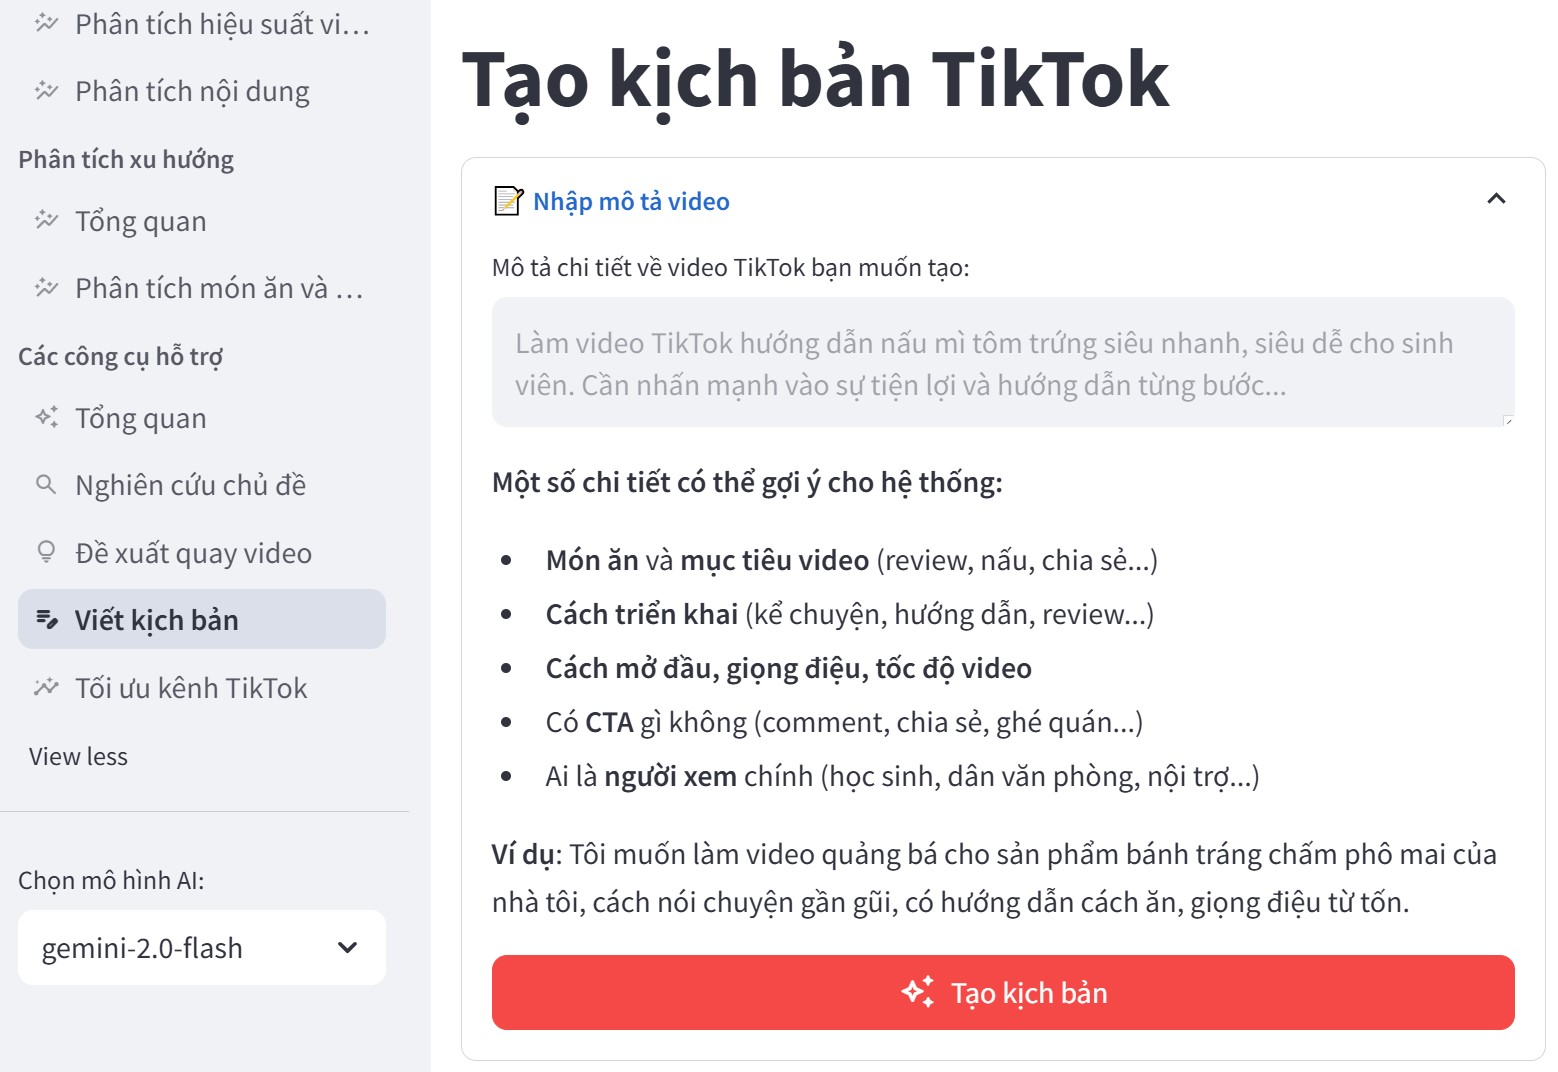
\includegraphics[width=0.99\linewidth]{img/21127739/scriptwriting/scriptwriting_main_page.jpg}}
    \caption{Giao diện chính của công cụ hỗ trợ viết kịch bản cho video TikTok}
    \label{fig:scriptwriting_main_page}
\end{figure}
